The Standard Model of particle physics (SM) describes various phenomena of particle physics.
The discovery of the Higgs boson ($H$) by the ATLAS and CMS collaboration at CERN completes the missing part of the SM prediction~\cite{Aad:2012tfa, Chatrchyan:2012xdj}.
However, there are several open challenges that cannot be explained by the SM, such as hierarchy problem~\cite{Weinberg:1975gm, Gildener:1976ai, Susskind:1978ms} and the dark matter candidate.
In order to answer those questions, a new theory extending the SM is necessary.
Supersymmetry (SUSY)~\cite{Wess:1973kz, Wess:1974tw, Golfand:1971iw, Martin:1997ns} is the most promising extensions of the SM.
SUSY, which is a spacetime symmetry, introduces the superpartners of SM particles (sparticles) with spin differing by one-half unit with respect to the SM partners.
The sparticles provide a potential solution to the hierarchy problem.
If $R$-parity is conserved~\cite{Fayet:1976et, Fayet:1977yc, Farrar:1978xj}, the sparticles are produced in pairs and the lightest SUSY particle (LSP) is stable providing the candidate for dark matter.

The charginos $\widetilde{\chi}^{\pm}_{1,2}$ and neutralinos $\widetilde{\chi}^{0}_{1,2,3,4}$ are the mass eigenstates in the order of increasing masses and collectively referred to as electroweakinos.
They are the mixture of the bino $\widetilde{B}$, winos $\widetilde{W}$, and Higgsinos $\widetilde{H}_{u,d}$ which are the superpartners of the $U(1)$, $SU(2)$ gauge bosons, and the Higgs bosons, respectively.
The charginos and neutralinos can decay into leptons and LSPs via $W$, $Z$, $H$ or sleptons $\widetilde{\ell}$.
In many SUSY models, the lightest neutralino $\widetilde{\chi}^{0}_{1}$ is the LSP.
The LSP couldn't be detected and results in significant missing transverse energy \MET.

The compressed scenarios refer to the small mass differences between heavier SUSY particles and the LSP.
For example, the mass differences between the heavier electroweakino states $\widetilde{\chi}^{0}_{2}$, $\widetilde{\chi}^{\pm}_{1}$ and the wino- or Higgsino-dominated LSP $\widetilde{\chi}^{0}_{1}$ range from a few {\MeV} to tens of {\GeV} depending on the composition of the mixture.
The $\widetilde{B}$, $\widetilde{W}$, and $\widetilde{H}$ composition of the $\widetilde{\chi}^{0}_{1}$ have an influence on the degree of compression.
Figure~\ref{fig:intro_LSP_composition} shows the composition of the lightest neutralino in a MSSM scan of the electroweakino sector~\cite{Aaboud:2016wna}.
Based on naturalness arguments~\cite{Barbieri:1987fn, deCarlos:1993rbr}, the Higgsino mass parameter $\mu$, the bino and wino mass parameters $M_{1}$ and $M_{2}$ satisfy $|\mu| \ll |M_{1}|, |M_{2}|$ leading to the three electroweakinos $\widetilde{\chi}^{0}_{1}$, $\widetilde{\chi}^{\pm}_{1}$, and $\widetilde{\chi}^{0}_{2}$ being dominated by the Higgsino.

\begin{figure}[htbp]
    \begin{center}
        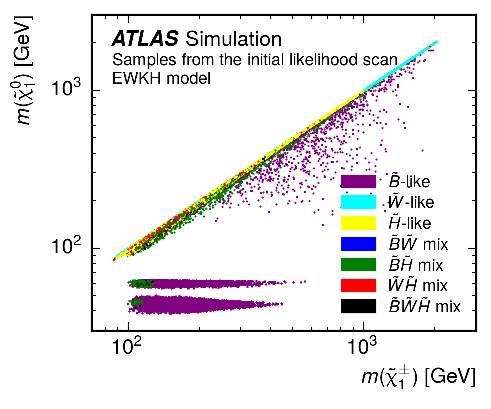
\includegraphics[scale=1.0]{LSP_composition.pdf}
        \caption{The scatter plot in the $m(\widetilde{\chi}^{0}_{1})$ vs $m(\widetilde{\chi}^{\pm}_{1})$ plane.
        The color encode the $\widetilde{\chi}^{0}_{1}$ composition.
        The Higgsino-dominated LSPs are colored in yellow and along the $\widetilde{\chi}^{0}_{1}$-$\widetilde{\chi}^{\pm}_{1}$ diagonal.
        The figure is taken from~\cite{Aaboud:2016wna}.}
        \label{fig:intro_LSP_composition}
    \end{center}
\end{figure}

This dissertation focuses on searching for electroweak production SUSY particles in compressed scenarios with exactly two low-momentum same-flavor opposite-charged leptons in final states and missing transverse momentum $\textbf{p}_{\text{T}}^{\text{miss}}$.
This search uses proton-proton collision data at $\sqrt{s} = 13$~{\TeV} recorded by the ATLAS detector at the Large Hadron Collider (LHC)~\cite{Evans:2008zzb} in 2015 and 2016, corresponding to a total integrated luminosity of 36.1~\ifb.
Figure~\ref{fig:intro_feynman_diagrams} shows the Feynman diagrams representing the electroweakino productions with two leptons final state in association with an initial state radiated jet.
Same-flavor opposite-charged leptons come from the $\widetilde{\chi}^{0}_{2}$ decays in the $\widetilde{\chi}^{0}_{2} \widetilde{\chi}^{\pm}_{1}$ and $\widetilde{\chi}^{0}_{2} \widetilde{\chi}^{0}_{1}$ productions, and from the $\widetilde{\chi}^{\pm}_{1}$ decays in $\widetilde{\chi}^{\pm}_{1} \widetilde{\chi}^{\mp}_{1}$ production.
The two leptons can be reconstructed in the detector and carry small transverse momentum  \pt hence they are very soft.
However, the two LSPs are invisible and back-to-back in the rest frame of their parent electroweakinos.
Because they carry large momentum, the missing transverse energy \met is relatively large.

Similar searches have been performed using $\sqrt{s} = 8$~{\TeV} and $\sqrt{s} = 13$~{\TeV} by the ATLAS~\cite{Aad:2014vma, Aad:2014nua, Aad:2015eda, Aaboud:2016wna} and CMS~\cite{Khachatryan:2014qwa, Khachatryan:2015pot, Sirunyan:2017lae} experiments.
Combining with the results from the LEP experiments, the mass limits for sleptons and charginos are $m(\widetilde{e}_{R}) > 73$~{\GeV}, $m(\widetilde{\mu}_{R}) > 94.6$~{\GeV}, and $m(\widetilde{\chi}^{\pm}_{1}) > 103.5$~{\GeV} or 92.4~{\GeV} depending on the $\Delta m(\widetilde{\chi}^{0}_{1}, \widetilde{\chi}^{\pm}_{1})$.

\begin{figure}[htbp]
    \begin{center}
        \begin{subfigure}[b]{0.32\textwidth}
            \begin{center}
                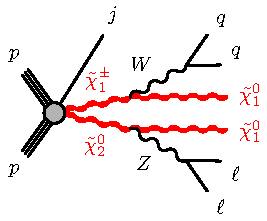
\includegraphics[scale=1.0]{C1N2-llqqN1N1g-WZ.pdf}
                \caption{The $\widetilde{\chi}^{0}_{2} \widetilde{\chi}^{\pm}_{1}$ production.}
            \end{center}
        \end{subfigure}%
        \begin{subfigure}[b]{0.32\textwidth}
            \begin{center}
                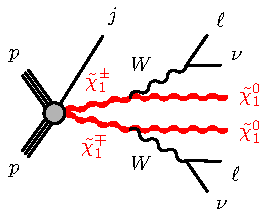
\includegraphics[scale=1.0]{C1C1-llvvN1N1g-WW.pdf}
                \caption{The $\widetilde{\chi}^{\pm}_{1} \widetilde{\chi}^{\mp}_{1}$ production.}
            \end{center}
        \end{subfigure}
        \begin{subfigure}[b]{0.32\textwidth}
            \begin{center}
                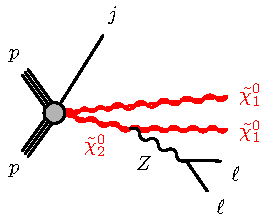
\includegraphics[scale=1.0]{N2N1-jllN1N1-Z.pdf}
                \caption{The $\widetilde{\chi}^{0}_{2} \widetilde{\chi}^{0}_{1}$ production.}
            \end{center}
        \end{subfigure}
    \end{center}
    \caption{The Feynman diagrams representing the two leptons final state of (a) $\widetilde{\chi}^{0}_{2} \widetilde{\chi}^{\pm}_{1}$, (b) $\widetilde{\chi}^{\pm}_{1} \widetilde{\chi}^{\mp}_{1}$, (c) $\widetilde{\chi}^{0}_{2} \widetilde{\chi}^{0}_{1}$ productions.}
    \label{fig:intro_feynman_diagrams}
\end{figure}

This dissertation has the following structure.
After introducing the theoretical foundations in the Chapters~\ref{chapter:standard_model} and \ref{chapter:Suppersymmetry}, the experiment facilities are described in Chapter~\ref{chapter:altas_experiment}.
The data and Monte Carlo samples used in this analysis are detailed in Chapter~\ref{chapter:data}.
The event reconstruction and selection are outlined in Chapter~\ref{chapter:event_reconstruction_and_selection}.
The background estimation and the systematic uncertainties are addressed in Chapter~\ref{chapter:bkg_estimation}.
Finally, the results and the conclusions are presented in Chapter~\ref{chapter:results} and Chapter~\ref{chapter:conclusion}.
The search for strongly-produced SUSY particles in final states with two same-sign or three lepton and jets (SS/3L+jets) were also studied and the detail can be found in App.~\ref{app:ss3l}.
